\documentclass[a4paper,11pt,exos]{nsi} 
\usepackage{fontawesome5}

%\pagestyle{empty}


\begin{document}



%\textcolor{UGLiBlue}{Mercredi 05/02/2025}\\
\classe{\terminale Comp}
\titre{Préparation de l'évaluation-bilan 7}
\maketitle

\exo{}
Calculer $\displaystyle \int_{0}^{2} \left ( 10e^{2x}+1 \right ) \ dx$.



\exo{}
Afin de chauffer un liquide, on fait passer un courant électrique dans une résistance.\\
La température, en °C, du liquide à l'instant $t$, en secondes, est noté $T(t)$.\\
On admet que la fonction $T$, définie sur $\fif{0}{80}$, est solution de l'équation différentielle :
$$(E) \quad T'=-0{,}02T+1$$
\begin{enumerate}
    \item Interpréter l'information $T(0)=20$.
    \item Résoudre $(E)$ sur $\fif{0}{80}$.
    \item Déterminer la solution de $(E)$ qui vérifie la condition initiale $T(0)=20$.
    \item Déterminer l'instant $t_0$, en s, à partir duquel la température du liquide dépasse 40 °C. \textit{On arrondira au dixième de seconde.}
\end{enumerate}



\exo{}
Lors d'une randonnée dans une région montagneuse, Jenny a mesuré à différentes reprises, l'altitude $a_i$ (en km) à laquelle elle se trouvait et la température $t_i$ (en °C).\\
\begin{center}
    \tabstyle[UGLiBlue]
    \begin{tabular}{|c|c|c|c|c|c|}
        \hline
        \ccell $a_i$ & 0,4 & 0,8 & 1,2 & 1,6 & 2 \\
        \hline
        \ccell $t_i$ & 8,4 & 6,2 & 3 & 0,2 & $-$2 \\
        \hline
    \end{tabular}
\end{center}
\begin{enumerate}
    \item À l'aide de la calculatrice, déterminer le coefficient de corrélation linéaire entre les deux variables $a$ et $t$. \textit{Arrondir au millième.}
    \item Peut-on envisager un ajustement affine de ce nuage de point ?\\
    Si oui, donner l'équation de la droite de régression de $t$ en $a$.
    \item Estimer alors la température à 2500 m d'altitude.
\end{enumerate}


\newpage

\setcounter{section}{0}

\classe{\terminale Comp}
\titre{Préparation de l'éval-bilan 7 - Corrigé}
\maketitle

\exo{}
Calculer $\displaystyle \int_{0}^{2} \left ( 10e^{2x}+1 \right ) \ dx$.

\textcolor{UGLiBlue}{
    \begin{enumerate}[label=\textbullet]
        \item On cherche une primitive $F$ de la fonction $f$ définie sur $\fif{0}{2}$ par $f(x) = 10e^{2x}+1$ :
        \begin{tabbing}
            Pour tout $x\in \fif{0}{2},\quad f(x)$ \= $= 10e^{2x}+1$\\
            \> $= 5\times 2 e^{2x} + 1$
        \end{tabbing}
        On pose : pour tout $x \in \fif{0}{2}$, $\quad$ $F(x) = 5e^{2x} + x$
        \item On calcule l'intégrale :
        \begin{tabbing}
            $\displaystyle\int_{0}^{2} \left ( 10e^{2x}+1 \right ) \ dx$ \= $= F(2) - F(0)$\\
            \> $= \left ( 5e^{2\times 2} + 2 \right ) - \left ( 5e^{0} + 0 \right )$\\
            \> $= 5e^{4} + 2 - 5$\\
            \> $= 5e^{4} - 3$
        \end{tabbing}
    \end{enumerate}
}

\exo{}
Afin de chauffer un liquide, on fait passer un courant électrique dans une résistance.\\
La température, en °C, du liquide à l'instant $t$, en secondes, est noté $T(t)$.\\
On admet que la fonction $T$, définie sur $\fif{0}{80}$, est solution de l'équation différentielle :
$$(E) \quad T'=-0{,}02T+1$$
\begin{enumerate}
    \item Interpréter l'information $T(0)=20$.
    \item Résoudre $(E)$ sur $\fif{0}{80}$.
    \item Déterminer la solution de $(E)$ qui vérifie la condition initiale $T(0)=20$.
    \item Déterminer l'instant $t_0$, en s, à partir duquel la température du liquide dépasse 40 °C. \textit{On arrondira au dixième de seconde.}
\end{enumerate}

\textcolor{UGLiBlue}{
    \begin{enumerate}
        \item La température du liquide à l'instant $t=0$ est de 20 °C.
        \item On résout l'équation différentielle $(E)$ :
        \begin{enumerate}[label=\textbullet]
            \item \textbf{Recherche d’une solution particulière constante :}\\
            Soit $T_0$ une solution particulière constante de $(E)$.\\
            On a donc : $T_0' = 0$ et $-0{,}02T_0 + 1 = 0$.\\
            On en déduit : $T_0 = \dfrac{1}{0{,}02} = 50$.
            \item \textbf{Recherche des solutions de l'équation homogène :}\\
            On résout l'équation différentielle $T'=-0{,}02T$ :\\
            Les solutions de cette équation homogène sont les fonctions définies sur $\fif{0}{80}$ par :
            $$T(t) = ke^{-0{,}02t}$$
            avec $k \in \R$.
            \item \textbf{Conclusion:}\\
            Les solutions de $(E)$ sont donc les fonctions définies sur $\fif{0}{80}$ par :
            $$T(t) = ke^{-0{,}02t} + 50$$
            avec $k \in \R$.
        \end{enumerate}
        \item Soit $T$ la solution de $(E)$ telle que $T(0)=20$.
        \begin{tabbing}
            $T(0)=20 \quad$ \= $\iff\quad ke^{-0{,}02\times 0} + 50 = 20$\\
            \> $\iff\quad k + 50 = 20$\\
            \> $\iff\quad k = 20 - 50$\\
            \> $\iff\quad k = -30$
        \end{tabbing}
        Donc la solution $T$ de $(E)$ telle que $T(0)=20$ est la fonction définie sur $\fif{0}{80}$ par :
        $$T(t) = -30e^{-0{,}02t} + 50$$
        \item On cherche l'instant $t_0$, en s, à partir duquel la température du liquide dépasse 40 °C.\\
        On résout donc l'inéquation : $T(t) > 40$
        \begin{tabbing}
            $T(t) > 40 \quad$ \= $\iff\quad -30e^{-0{,}02t} + 50 > 40$\\
            \> $\iff\quad -30e^{-0{,}02t} > 40 - 50$\\
            \> $\iff\quad -30e^{-0{,}02t} > -10$\\
            \> $\iff\quad e^{-0{,}02t} < \dfrac{1}{3}$\\
            \> $\iff\quad -0{,}02t < \ln\left(\dfrac{1}{3}\right)$\\[.5em]
            \> $\iff\quad t > -\dfrac{\ln\left(\dfrac{1}{3}\right)}{0{,}02}$\\[.5em]
            \> $\iff\quad t > -\dfrac{-\ln(3)\times 50}{0,02\times 50}$\\[.5em]
            \> $\iff\quad t > 50\ln(3)$    
        \end{tabbing}
        La valeur approchée de $t_0=50\ln(3)$ est $t_0 \approx 54{,}9$ s.\\
        Donc la température du liquide dépasse 40 °C à partir de l'instant $t_0 \approx 54{,}9$ s.
    \end{enumerate}
}

\exo{}
Lors d'une randonnée dans une région montagneuse, Jenny a mesuré à différentes reprises, l'altitude $a_i$ (en km) à laquelle elle se trouvait et la température $t_i$ (en °C).\\
\begin{center}
    \tabstyle[UGLiBlue]
    \begin{tabular}{|c|c|c|c|c|c|}
        \hline
        \ccell $a_i$ & 0,4 & 0,8 & 1,2 & 1,6 & 2 \\
        \hline
        \ccell $t_i$ & 8,4 & 6,2 & 3 & 0,2 & $-$2 \\
        \hline
    \end{tabular}
\end{center}
\begin{enumerate}
    \item À l'aide de la calculatrice, déterminer le coefficient de corrélation linéaire entre les deux variables $a$ et $t$. \textit{Arrondir au millième.}
    \item Peut-on envisager un ajustement affine de ce nuage de point ?\\
    Si oui, donner l'équation de la droite de régression de $t$ en $a$.
    \item Estimer alors la température à 2500 m d'altitude.
\end{enumerate}

\textcolor{UGLiBlue}{
    \begin{enumerate}
        \item On utilise la calculatrice pour déterminer le coefficient de corrélation linéaire entre les deux variables $a$ et $t$ :
        \begin{center}
            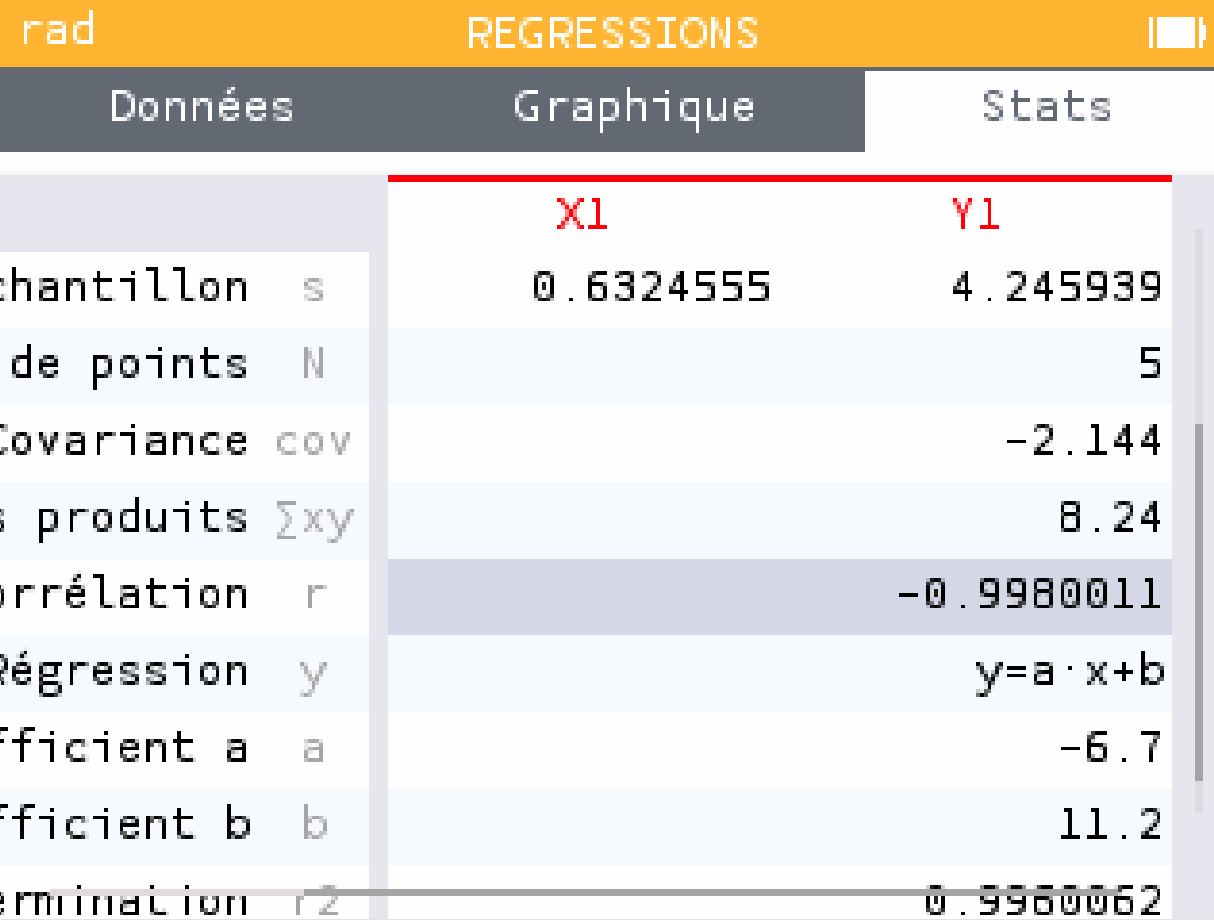
\includegraphics[width=6cm]{corr_stat.png}
        \end{center}
        $$r \approx -0{,}998$$
        \item La coefficient de corrélation est proche de $-1$, on peut envisager un ajustement affine de ce nuage de point.\\
        L'équation de la droite de régression de $t$ en $a$ est :
        $$t = -6,7a + 11,2$$
        \item Pour estimer la température à 2500 m (soit 2,5 km) d'altitude, on remplace $a$ par 2,5 dans l'équation de la droite de régression :
        $$t = -6,7\times 2{,}5 + 11,2 = -5{,}55$$
        Donc on peut estimer la température à 2500 m d'altitude à environ $-5{,}55$ °C.
    \end{enumerate}
}
\end{document}


\textbf{Dans cet exercice, les questions 1, 2, 3 et 4 peuvent être traitées de façon indépendante les unes des autres.}

Un parachutiste est en chute libre dans l'air jusqu'à l'instant $t = 0$ où il ouvre son parachute. Sa vitesse est alors de 50~m.s$^{-1}$. On admet par la suite que sa vitesse $v$, en m.s$^{-1}$, en fonction du temps $t$, en $s$, est solution de l'équation différentielle sur l'intervalle $[0\;;\;+\infty[$:

\[(E)\;:\quad y'=-5y+10.\]


\begin{flushleft}
\textbf{Question 1}
\end{flushleft}

La fonction constante $g$ définie sur l'intervalle $[0\;;\;+\infty[$ par $g(t)=2$ est-elle une solution de l'équation différentielle $(E)$ ? 
Justifier la réponse.

\begin{flushleft}
\textbf{Question 2}
\end{flushleft}

Montrer que les solutions de l'équation différentielle $(E)$ sur l'intervalle $[0\;;\;+\infty[$ sont les fonctions $f$ définies sur cet intervalle par $f(t)=k\e^{-5t}+2$, où $k$ est un nombre réel donné.

\begin{flushleft}
\textbf{Question 3}
\end{flushleft}

En admettant le résultat de la question précédente, montrer que la fonction $v$ est donnée sur $[0\;;\;+\infty[$ par $v(t) = 48 \e^{-5t} + 2$.

\begin{flushleft}
\textbf{Question 4}
\end{flushleft}

La distance parcourue, en mètre, par le parachutiste pendant les 10 premières secondes après ouverture du parachute est donnée  par l'intégrale :

\[\displaystyle\int_{0}^{10} \left ( 48 \e^{-5t} +2 \right ) \ dt\]

Calculer cette intégrale (arrondir à $10^{-1}$).

\begin{flushleft}
\textbf{Question 1}
\end{flushleft}

Soit $g$ la fonction constante définie sur l'intervalle $[0\;;\;+\infty[$ par $g(t)=2$.

$g'(t)=0$ et $-5g(t)+10=-5\times 2 +10=0$ donc $g'(t)=-5g(t)+10$.

Donc $g$ est solution de l'équation différentielle $(E)$.

\begin{flushleft}
\textbf{Question 2}
\end{flushleft}

D'après le cours, les solutions de l'équation différentielle $y'=ay$ sur l'intervalle $[0\;;\;+\infty[$ sont les fonctions $f$ définies sur cet intervalle par $f(t)=k\e^{at}$,  où $k$ est un nombre réel quelconque, donc les solutions de l'équation différentielle $y'=-5y$ sur l'intervalle $[0\;;\;+\infty[$ sont les fonctions $f$ définies sur cet intervalle par $f(t)=k\e^{-5t}$,  où $k$ est un nombre réel quelconque.

Une solution de l'équation différentielle $y'=-5y+10$ est la somme d'une solution de l'équation différentielle $y'=-5y$ et d'une solution constante de l'équation différentielle $y'=-5y+10$, donc les solutions de l'équation différentielle $(E)$ sur l'intervalle $[0\;;\;+\infty[$ sont les fonctions $f$ définies sur cet intervalle par $f(t)=k\e^{-5t}+2$,  où $k$ est un nombre réel quelconque.

\begin{flushleft}
\textbf{Question 3}
\end{flushleft}

On sait que $v$ est solution de $(E)$ et que $v(0)=50$; donc $k\e^{0}+2 = 50$ donc $k=48$.

La fonction $v$ est donc donnée sur $[0\;;\;+\infty[$ par $v(t) = 48 \e^{-5t} + 2$.

\begin{flushleft}
\textbf{Question 4}
\end{flushleft}

La distance parcourue, en mètre, par le parachutiste pendant les 10 premières secondes après ouverture du parachute est donnée  par l'intégrale:
$\displaystyle\int_{0}^{10} \left ( 48 \e^{-5t} +2 \right ) \d t$.

Pour calculer cette intégrale, il faut trouver une primitive de la fonction $v$.

La fonction $t\longmapsto \e^{at}$ avec $a\neq 0$,  a pour primitive la fonction $t\longmapsto \dfrac{\e^{at}}{a}$, donc la fonction $v$ a pour primitive la fonction $V$ définie par $V(t) = 48 \dfrac{\e^{-5t}}{-5} + 2t$ soit $V(t) = - 9,6 \e^{-5t} +2t$.

$\begin{aligned}
\displaystyle\int_{0}^{10} \left ( 48 \e^{-5t} +2 \right ) \ dt&
= \left [ V(t) \strut\right ]_{0}^{10}
= V(10) - V(0)
= \left (-9,6 \e^{-5\times 10} + 2 \times 10 \right ) - \left ( -9,6 \e^{-5\times 0} + 2 \times 0 \right )\\
&
= -9,6 \e^{-50} + 20+9,6  = 29,6 -9,6 \e^{-50} \approx 29,6
\end{aligned}$


\end{document}